\documentclass[12pt]{article}
\usepackage[english]{babel}
\usepackage{natbib}
\usepackage{url}
\usepackage[utf8x]{inputenc}
\usepackage{amsmath}
\usepackage{graphicx}
\graphicspath{{images/}}
\usepackage{parskip}
\usepackage{fancyhdr}
\usepackage{vmargin}
\setmarginsrb{3 cm}{2.5 cm}{3 cm}{2.5 cm}{1 cm}{1.5 cm}{1 cm}{1.5 cm}

% Template started from: https://www.overleaf.com/latex/templates/uct-report-template/grctkzjtrqrm

\title{Course Project}										% Title
\author{Grant Atkins\\Devin Haslam}							%Authors
\date{\today}											% Date

\makeatletter
\let\thetitle\@title
\let\theauthor\@author
\let\thedate\@date
\makeatother

%\pagestyle{fancy}
%\fancyhf{}
%\rhead{\theauthor}
%\lhead{\thetitle}
%\cfoot{\thepage}

\begin{document}

%%%%%%%%%%%%%%%%%%%%%%%%%%%%%%%%%%%%%%%%%%%%%%%%%%%%%%%%%%%%%%%%%%%%%%%%%%%%%%%%%%%%%%%%%

\begin{titlepage}
	\centering
    \vspace*{0.5 cm}
    
\includegraphics[scale = 1.8]{ODU.png}\\[1.0 cm]	% University Logo
    \textsc{\LARGE Old Dominion University}\\[2.0 cm]	% University Name
	\textsc{\Large CS 773}\\[0.5 cm]				% Course Code
	\textsc{\large Data Mining and Security}\\[0.5 cm]				% Course Name
	\rule{\linewidth}{0.2 mm} \\[0.4 cm]
	{ \huge \bfseries \thetitle}\\
	\rule{\linewidth}{0.2 mm} \\[1.5 cm]
	
	\begin{minipage}{0.4\textwidth}
		\begin{flushleft} \large
			\emph{Authors:}\\
			\theauthor
			\end{flushleft}
			\end{minipage}~
			\begin{minipage}{0.4\textwidth}
			\begin{flushright} \large
%			\emph{Student Number:} \\
%			XXXXXX000									% Your Student Number
		\end{flushright}
	\end{minipage}\\[2 cm]
	
	{\large \thedate}\\[2 cm]
 
	\vfill
	
\end{titlepage}

%%%%%%%%%%%%%%%%%%%%%%%%%%%%%%%%%%%%%%%%%%%%%%%%%%%%%%%%%%%%%%%%%%%%%%%%%%%%%%%%%%%%%%%%%

\tableofcontents
\pagebreak

%%%%%%%%%%%%%%%%%%%%%%%%%%%%%%%%%%%%%%%%%%%%%%%%%%%%%%%%%%%%%%%%%%%%%%%%%%%%%%%%%%%%%%%%%

\section{Executive Summary}

The goal of this course project, originally stemmed from Open University Learning Analytics data set, is to identify ``at-risk'' students 
provided \cite{oulad}. In order to simplify our data mining techniques we decided to use the classification ``fail'' in place of ``withdraw'' and ``pass'' in place of ``distinction.'' This should not effect the results of our methods because this will still help us identify ``at-risk'' students. 

We first analyzed the data given to find the most effective attributes. From this initial assessment we found that many attributes did not contribute to the final result of a student while other attributes had a large impact on the likelihood of passing or failing. Some of these important attributes were ``total clicks,'' ``scores,'' and ``dates.'' One might notice that our most useful attributes come from VLE results. We observed that the VLE provided more useful data than demographic information.

By visualizing the data, we have found some very useful statistics that can be used to improve the accuracy of models. Tables \ref{fig:chart} and \ref{table:dem_infogain} give important insight to which attributes are more important for our methods. Figures \ref{fig:click_vs_score} and \ref{fig:click_vs_score_f} display the practical correlation between click counts, score, and result. Another visualization, Figure \ref{fig:weightVSscore}, exhibits that failing students tend to perform similarly on certain assignments. All of this information was taken into account when creating our final model. 

Some of our effort was spent testing different combinations of data by combining certain files and removing useless attributes. In the end we found our best accuracy with two files, one for demographic and registration data, the other for VLE interaction data. From the demographic data we used k-means clustering to find clusters of students who are likely to pass or fail. On the other hand we will use a J48 decision tree on the VLE interaction data to predict the result of each student. Once we have VLE data, we have observed that we should no longer use the demographic data.

Our results show that we have created an accurate way to predict whether a student will pass or fail. We used and explored well known machine learning methods such as: naive bayes, decision trees and k-means to justify our results. Our method gives 87\% accuracy with a precision of 87\& and a recall of 96\%. While we acknowledge that this score could be improved, there are challenges extracting useful information from under utilized attributes such as "date." 

%This is a simple report template with the UCT logo. Feel free to use/modify it to suit your needs. Variables that need to be altered have been commented to make modifications easier. For example if you need to change the university logo, look for the comment \texttt{\% University Logo} in this file and then make appropriate modifications in that line.
%
%A Table of Contents and a bibliography have also been implemented. To add entries to your bibliography, simply edit \texttt{biblist.bib} in the root folder and then use the \texttt{\textbackslash cite\{\ldots\}} command in \texttt{main.tex} \cite{bibtex}. The Table of Contents will be updated automatically.
%
%I hope that you find this template both visually appealing and useful. \\

\newpage
\section{Introduction}

With analytics becoming an integral part of Learning Management Systems (LMS), Universities can analyze their data to intervene and aid ``at-risk'' 
students. This can be done by detecting failing or struggling students earlier on in their courses. These detections can later be used to predict ``at-risk''
students for future intervention. Analysis of demographic information for students may also prove useful to detect environments or character
attributes that identify a struggling group.

The Open University (OU) in the United Kingdom, offered distance learning courses with its virtual learning environment (VLE) from 2013 to 2014. Students interacted with 
the VLE and OU then collects information such as: page names, clicks, and times connected to the website. Students are also required to register for these 
courses earlier on, which provides: registration date, unregistration date, class types and semester. Many students may end up failing or withdrawing from the VLE 
courses. The data sets that OU provided can be used to provide insight on 2013 to 2014 semester students. 

\section{Problem Statement}

When analyzing students to observe for ``at-risk'' students it may seem easily done by looking at simply grade scores, however, there could be factors
present in a student's personal history or personal accomplishments that correlate with course problems causing a student to be ``at-risk.'' The goal of this paper is discuss and find data mining techniques that aid in the detection and prediction of ``at-risk'' students.

\section{Solution Methodology}

Finding a solution for this project was based on the data being observed. We first attempted to look at each data set, each csv provided, individually and then find attributes that would be the best indicators to determine the ``final\_result'' of students. The tools used for this project included weka, R and python. We used weka for classifying and clustering. We used R and python for merging data which is included in our public repository \cite{github}. Later we would merge the data sets together and then perform the following steps depending on the data set:

\begin{enumerate}
  \item Find the best attributes for the data provided, often through information gain for feature selection or PCA for clustering
  \item Test machine learning techniques such as:
  \begin{enumerate}
     \item Decision trees
     \item Naive bayes
     \item Bagging
     \item K-means
  \end{enumerate}
  \item Cross validation for measuring effectiveness
\end{enumerate}

This paper first experiments upon the individual data sets and then the results of the merged data sets as explained in the next section.

\section{Experimental setup and data used}

There are many different ways to experiment on the OU learning analytics data set. There are many interactions between the different sets of data, such as demographic
information can be linked to course assessments for each student as shown in Figure \ref{fig:db_model}. The attribute ``final\_result'' was the main attribute that was used in each data set because it determines whether students passed, failed, withdrawn or gained distinction. We found these attributes to be along the same lines, so we eventually paired them to Pass or Fail, where withdrawn became Fail and distinction became Pass.
 
 While each file may contain valuable information about a student, many times important details can be lost among large amounts of useless data. In our attempt to isolate the most important attributes, we ran the files that were correlated with a student passing or failing to find information gain. These four files, "studentAssessment", "studentInfo", "studentRegistration", and "studentVle" provided the most useful attributes to determine if a student passed or failed. The information gain for each of these files is displayed below in Tables 1 and 2. We found that the files "course" and "Vle" were almost completely useless. These files were not helpful to us due to the limited amount of information, and an inability to correlate the information with an individual student.  The last file "assessments," was not very useful, but we did include the weight of an assignment in our final combined file.
 
 From table 1, we learned valuable information about individual attributes when they are tested separatly. It was not a surprise to see that the scores that a student makes has an effect on whether they pass or not. From the "studentRegistration" file, we observed that "date\_unregistration" had a high information gain. This is also expected because we know that if a student is "unregistering" they are dropping out of the course and that it is too late to advise them. We therefore did not include this attribute in our combined file.
 
 When looking at the file "studentVle," it looks as if the amount of click does not have a large effect on whether the student passes or not. However, when calculating the total number of clicks that a student did across the semester we can much more accurately predict when a student might fail. In the combined file, it can be observed that the total number of clicks was the most important attribute.
 
 Originally we believed that combining the weight of an assignment with the score a student received, could provide vital information to data mining methods. However, after combining these files, it was observed that there was little to no improvement. Although it is clear that Exams are important to do well on, we did not see a linear correlation as the weight of the assignments decreased. We did decide to include the weight attribute in our final combined file due to the very small increase in accuracy observed.
 
 \begin{table}[h]
 \centering
 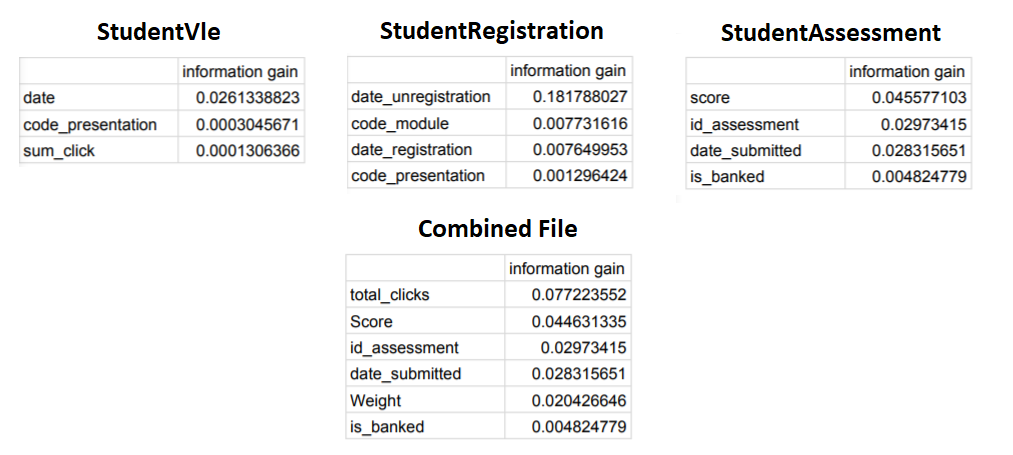
\includegraphics[scale=.75]{chart.png}
 \caption{Information gain of files related to students \cite{oulad}}
 \label{fig:chart}
 \end{table}
 
 \begin{figure}[h]
 \centering
 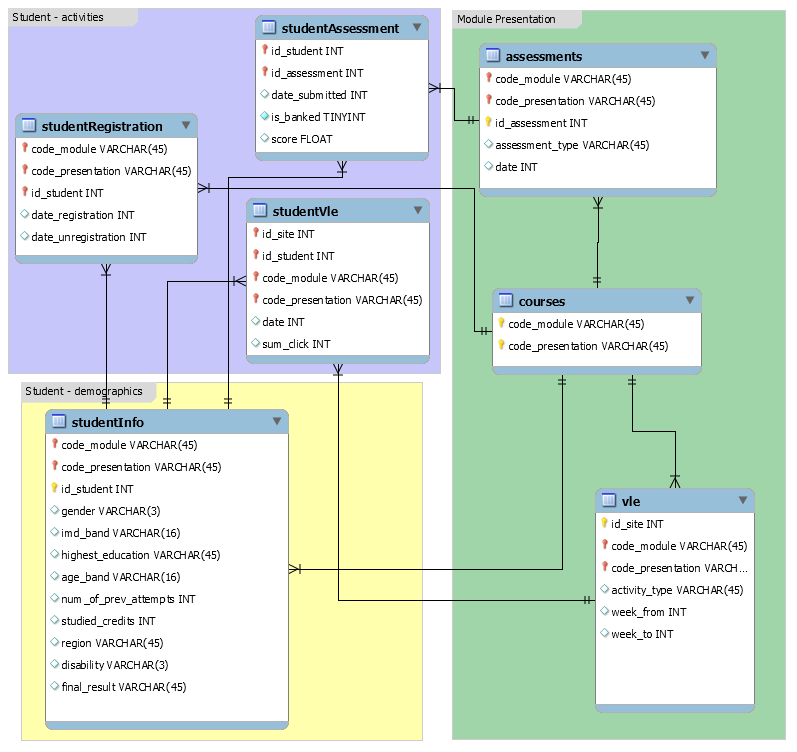
\includegraphics[scale=0.5]{db_model.png}
 \caption{OU learning analytics data set relations \cite{oulad}}
 \label{fig:db_model}
 \end{figure}

 When testing this data, non-important attributes were purged. For example, student\_id was removed because there is nothing to gain from specific individual students compared to other attributes such as score or code\_module where there can be correlations. 

 After purging useless material from the input, we used various data mining techniques on each file separately to see if we could accurately predict whether a student would pass or fail. While certain files such as "studentVle" and "studentAssessment" did produce good results, it was not until we combined several of these files that we observed the best outcome.  
 

\begin{figure}[h]
 \centering
 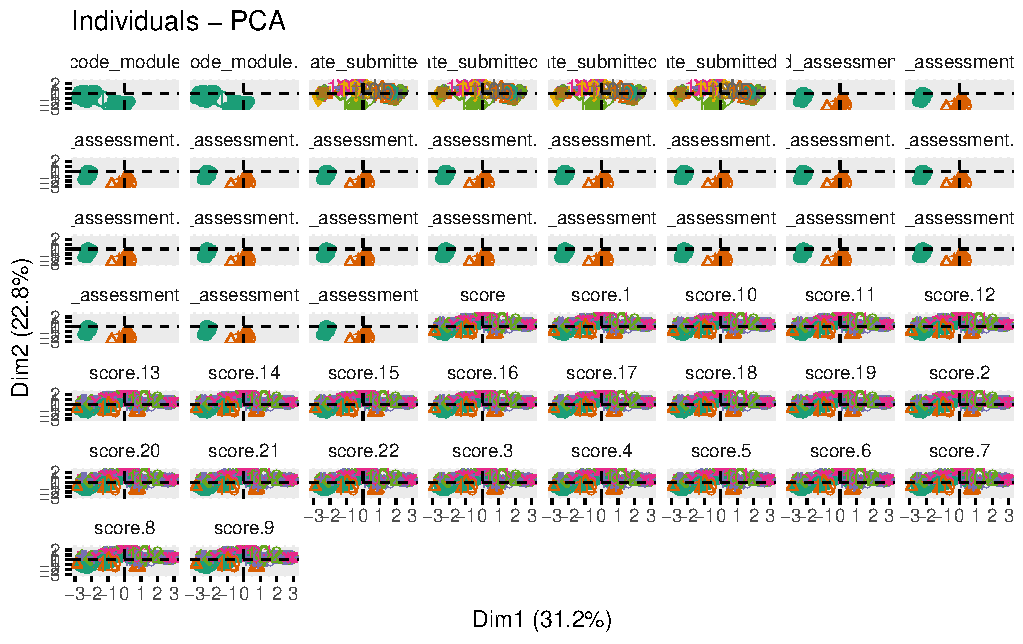
\includegraphics[scale=0.8]{PCA_Assessments_first50.pdf}
 \caption{PCA of student assessment attributes}
 \label{fig:pca}
 \end{figure}
 
 When first reviewing the data presented to us individually, student demographics was the first to be reviewed as this is information that is often received before a course has started. Approaching this set of data we first decided to use information gain to discover the best attributes to build a decision tree. This lead to interesting results as all of the attributes never had above a 5\% information gain as shown in table \ref{table:dem_infogain}. This result combined with poor accuracy when using data mining techniques deterred us away from using attributes from demographic information aside from final\_result, which is the classifier for this data set.
 
 
 \begin{table}
\centering
\begin{tabular}{ | l | l | l | p{7.8cm} | }
\hline
\textbf{Attribute} & \textbf{Information Gain} \\
\hline
code\_module & 0.0333132948 \\
\hline
studied\_credits & 0.0291538626 \\
\hline
highest\_education & 0.0220755496 \\
\hline
imd\_band & 0.0190484622 \\
\hline
date\_registration & 0.0126263112 \\
\hline
num\_of\_prev\_attempts & 0.0112197577 \\
\hline
region & 0.0099021067 \\
\hline
code\_presentation & 0.0090550367 \\
\hline
age\_band & 0.0047750479 \\
\hline
disability & 0.0030386879 \\ 
\hline
gender & 0.0003658152 \\
\hline

\end{tabular}
\caption{Information gain of student info and registration data merged}
\label{table:dem_infogain}
\end{table}

\section{Results}

Performing simple k-means using Weka's ``densityBasedClusterer'', showed very clear cluster when observing a students' click counts vs students' assessment scores as shown below in Figure \ref{fig:click_vs_score}.
K-means chose number of clicks as the best attribute to perform clustering on. 

We also attempted to use principal component analysis (PCA) on a merged set of data from a student's demographic information and assessment scores. Unfortunately finding PCA on all the different number of factors for each attribute is computationally taxing and time consuming, therefore we attempted PCA on the first 50 entries of this data set as shown in Figure \ref{fig:pca}. This attempted to find correlation between each of the factors of each attribute, where the more linear the graph was, the better correlation. As shown in Figure \ref{fig:pca}, we attempted to find correlations between code\_module, assessment type and student scores. It shows that scores had better correlations with many other attributes, which means it was better to cluster upon which proves true with Figure \ref{fig:click_vs_score}, with more explained below.

\begin{figure}[h]
 \centering
 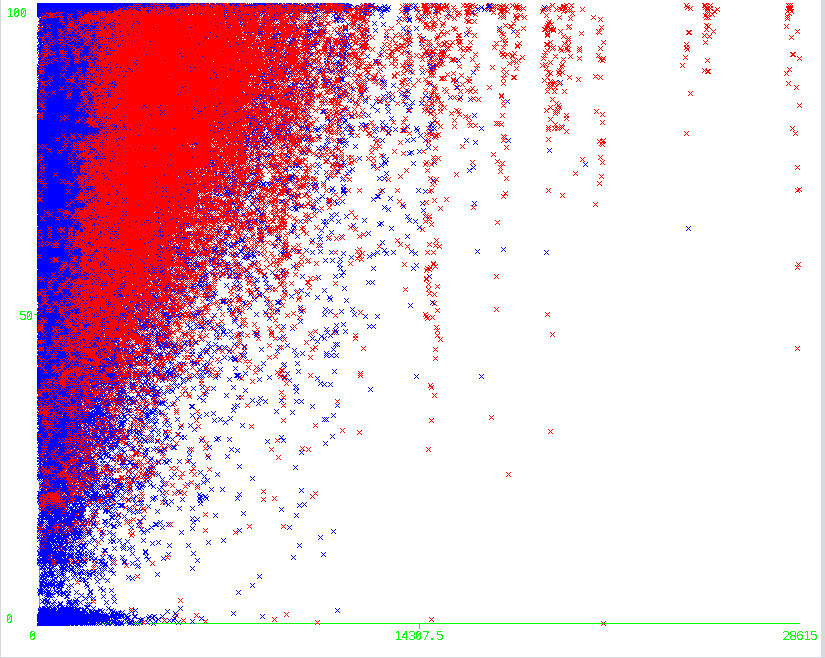
\includegraphics[scale=0.35]{click_count_vs_score_clusters.png}
 \caption{K-means clusters for click\_counts vs scores (Y-axis is score, X-axis is total click count)}
 \label{fig:click_vs_score}
 \end{figure}
 
 If we view the clusters as final results, it becomes apparent that there is a correlation between click counts and scores for determining if a student passes or fails in the end. After approximately 14,500 clicks in the content, students generally all pass, even if a student receives a failing score after as shown in Figure \ref{fig:click_vs_score_f}. 

\begin{figure}[h]
 \centering
 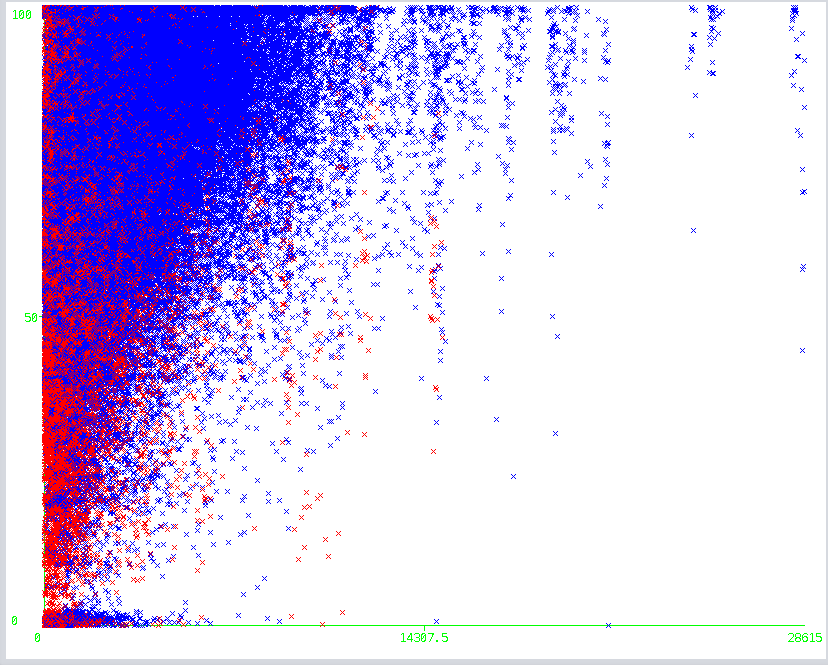
\includegraphics[scale=0.35]{click_count_vs_score_finalresults.png}
 \caption{K-means results for click\_counts vs scores with Blue being passing and red being failing (Y-axis is score, X-axis is total click count)}
 \label{fig:click_vs_score_f}
 \end{figure}

Students who took the highest weighted assignment, where weight was 100, and scored below a 50 had a 87.88\% chance to fail. This is fairly critical for students scores, stressing importance on these weighted tests, as shown in Figure \ref{fig:weightVSscore}.

Intuitively, the better a student does on an important assignment, the more likely they are to pass. From Figure \ref{fig:weightVSscore}, it becomes obvious that this idea holds up when looking at the data. As one might expect, the exam grade of a student had a large impact on their final grade in the class. When looking at less important assignments, the division between passing and failing students becomes less clear. It seems that failing students are most likely to pass assignments that are not weighted high or low, but are in the middle. From this information we can see that good students focus on both the important and unimportant assignments, while bad students are likely to do best on assignments that are weighted in the middle.

A second lesson we can learn from Figure \ref{fig:weightVSscore} pertains to getting a 0 on an assignment. If a student gets a 0 on the exam, there is obviously no hope for them passing. However, students can still pass the course if they receive a 0 on lower weighted assignments. Specifically, if a student does not turn in the lowest weighted assignments, there is still a good chance they can pass. This can be seen at the origin of the scatter plot where a large number of blue passing students can be seen. This is different from the rest of the assignments where a 0 means a very high likely hood of failing.

 \begin{figure}[h]
 \centering
 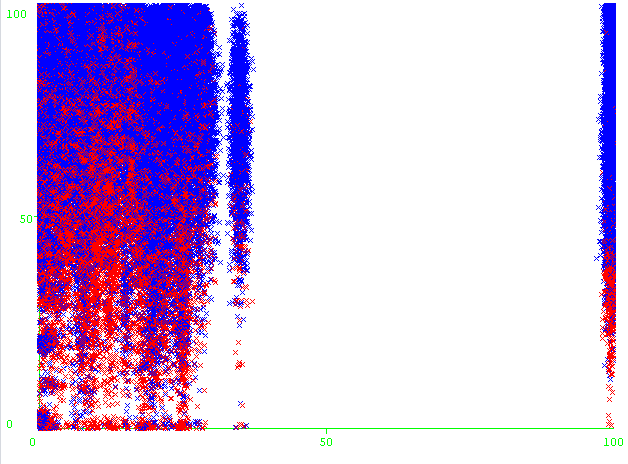
\includegraphics[scale =1]{weightscore.png}
 \caption{Correlation between weight of assignment and score on that assignment (Y-axis is score, X-axis is weight, red is fail, blue is pass)}
 \label{fig:weightVSscore}
 \end{figure} 

 
\clearpage
\section{Conclusions}

After exploring this large amount of data with various data mining techniques, we have learned a lot of useful information. One of the most obvious results is that demographic data is only useful before the course starts. As soon as students have access to the VLE, the demographic begins to become more less important. Using VLE data, we can create much more accurate predictions because we now know about the behavior of the students. 

When looking at the VLE data, some attributes are more important than others. From our experience, the total number of clicks seems to be the most important information recorded by the VLE. This is somewhat surprising, as one would usually assume that scores have more of an effect on whether a student will pass or fail. We rationalize this phenomenon by suggesting that amount of clicks has a heavy correlation with knowledge gained and work ethic of the student. The date a student accesses the VLE also has a large impact on the final grade. Proactive students who explore the VLE before the course has started find a 67\% passing rate. 

In a real life situation, we must predict a student's results in real time. Before a course starts, we propose that a k-means clustering routine should be performed on past demographic and registration data. If the student has clicked before the course has started, we also include this information in the clustering. We would then compare each new student to these clusters and create a list of student that are most likely to fail. Depending on the resources of the university, a certain percentage of these dangerous students would be preliminary advised. After the course starts, we would not pay attention to theses clusters as much anymore. We then propose that a decision tree would be created to analyze the most important VLE data weekly. Some of these important attributes include total clicks, date of clicks, scores, weights, unique days accessed, and days since last access. We believe this is the most effective way to advise students.

Although we did not analyze the students weekly with attributes such as days since last access, we could still accurately predict a student based on our combined file of attributes. We could not include all effective attributes in this file, but this combined file contains most of the important data. Just from this file, we can use a simple J48 decision tree to get 87\% accuracy. Depending on the size of the training set data, the decision tree accuracy can be increased even more as it will eventually recognize very common characteristics of different attributes. We know that this could be improved even further if we did a careful analysis of dates that the course was accessed. At the moment we are only using the date\_submitted attribute which is not quite as effective. Despite this, we can still accurately predict if a student is going to pass or fail the course with small error.

When looking at the results of this method it is important to also look at the precision and recall of the decision tree. For this problem, it is more important to wrongfully classify a failing student as passing than a passing student as failing. If a failing student is classified as passing, this is because the student must be doing something correctly. Although it is unfortunate that this student may not get counseling, many failing students wont be able to get counseling due to the resources of the university. There are other students who need the counseling more than a failing student classified as passing. On the other hand, if passing students are labeled as failing, this is a more detrimental outcome. In this case, resources will be wasted counseling this passing student and will mean that other failing students wont be able to receive the needed help. When applying this idea to precision and recall, this means that recall is more important than precision. In our decision tree, we had a precision of 87\% but a recall of 96\%. This means that our result is well suited to the problem at hand. 


%\hspace{1 cm}--- End

\clearpage
\bibliographystyle{plain}
\bibliography{biblist}

\end{document}